\chapter{Subsystem Integration}\label{ch:integration}

\begin{tipbox}[When to Read This Chapter]
\textbf{Sprint~3}: Skim the integration sequence and N\textsuperscript{2} diagram sections to inform your CDR interface definitions. \textbf{Sprint~4}: Read the full chapter before starting subsystem demonstrations. \textbf{Sprints~5--6}: Return to the debugging and configuration management sections during system integration.
\end{tipbox}

\begin{warningbox}[Integration Time Estimate]
Integration always takes longer than expected. Plan for integration to consume 30--50\% of total project time. If your Gantt chart shows one week for integration, double it. The most common schedule failure in student projects is underestimating integration effort. See Chapter~20 (p.\,\pageref{ch:debug}) for the systematic debugging methodology you will need when integration reveals faults.
\end{warningbox}

\vspace{1em}
\vspace{1em}

\begin{figure}[htbp]\centering
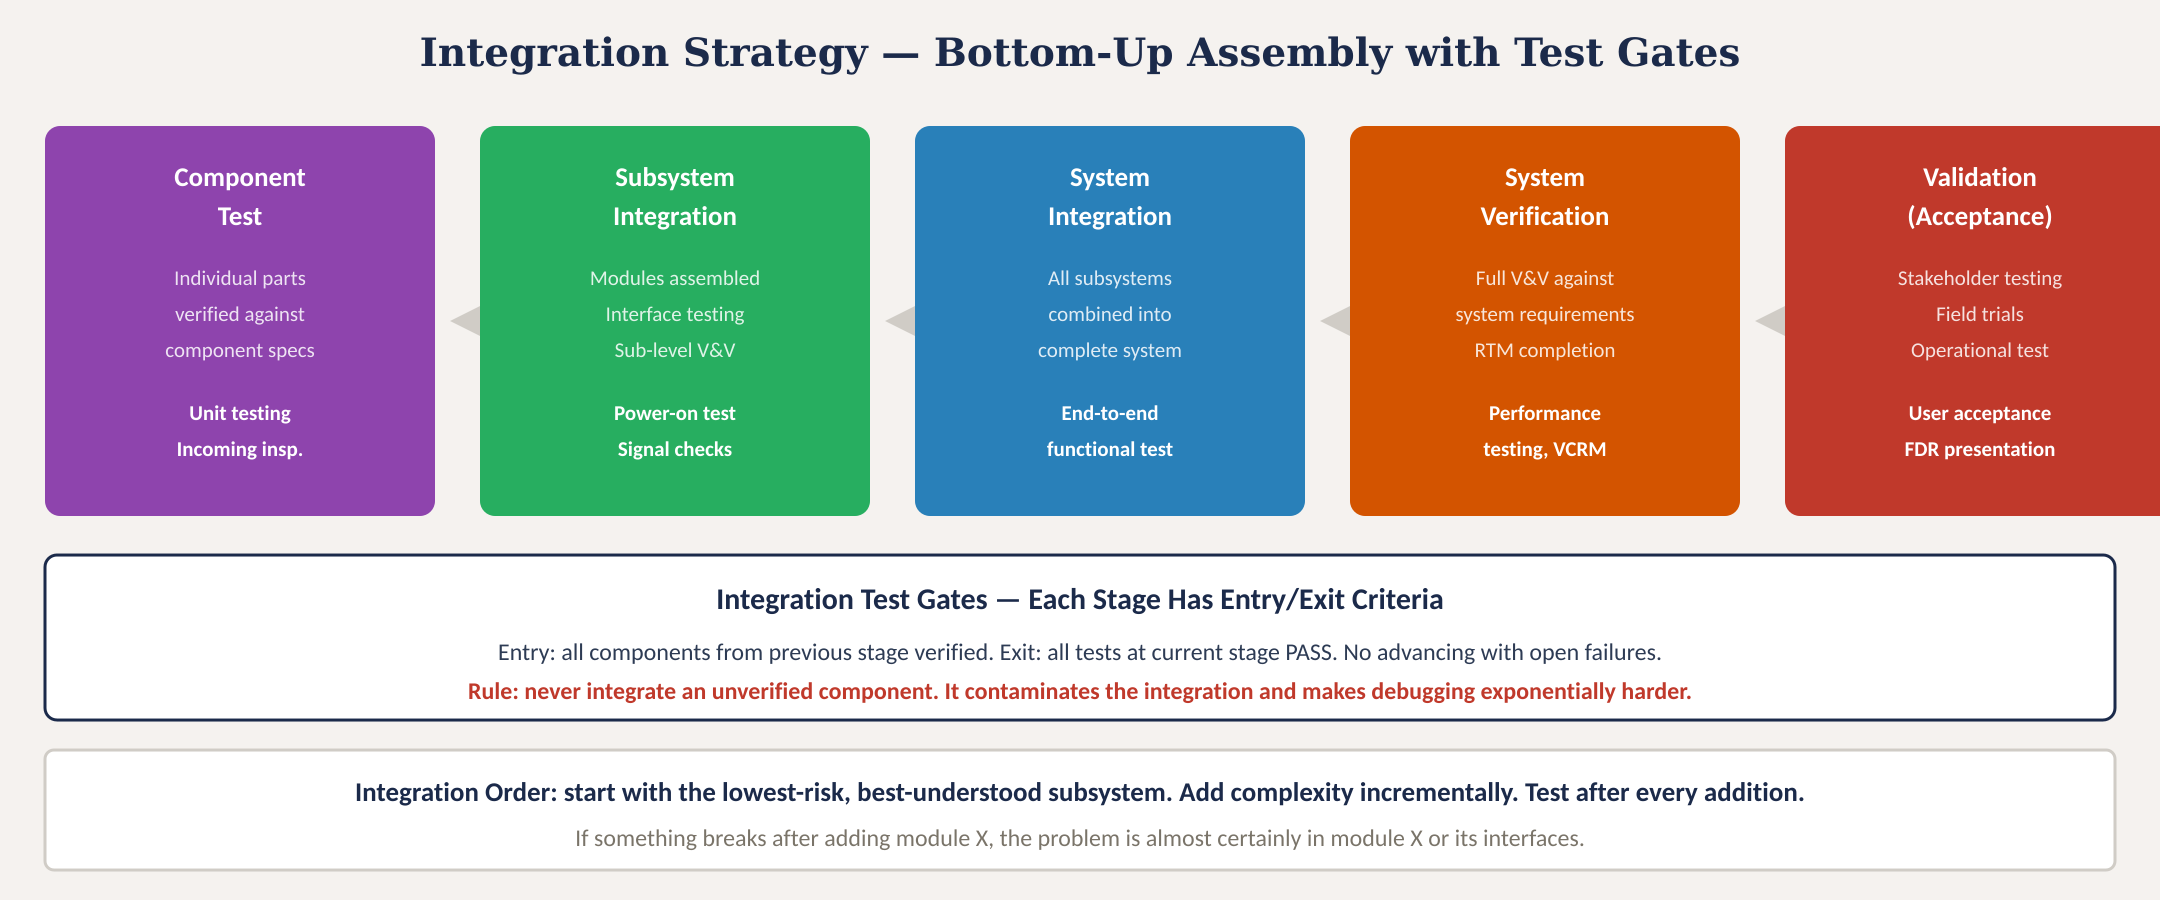
\includegraphics[width=\textwidth]{master_figs/fig_integration_strategy.png}
\caption{Bottom-up integration with test gates.}\end{figure}

\begin{figure}[htbp]\centering
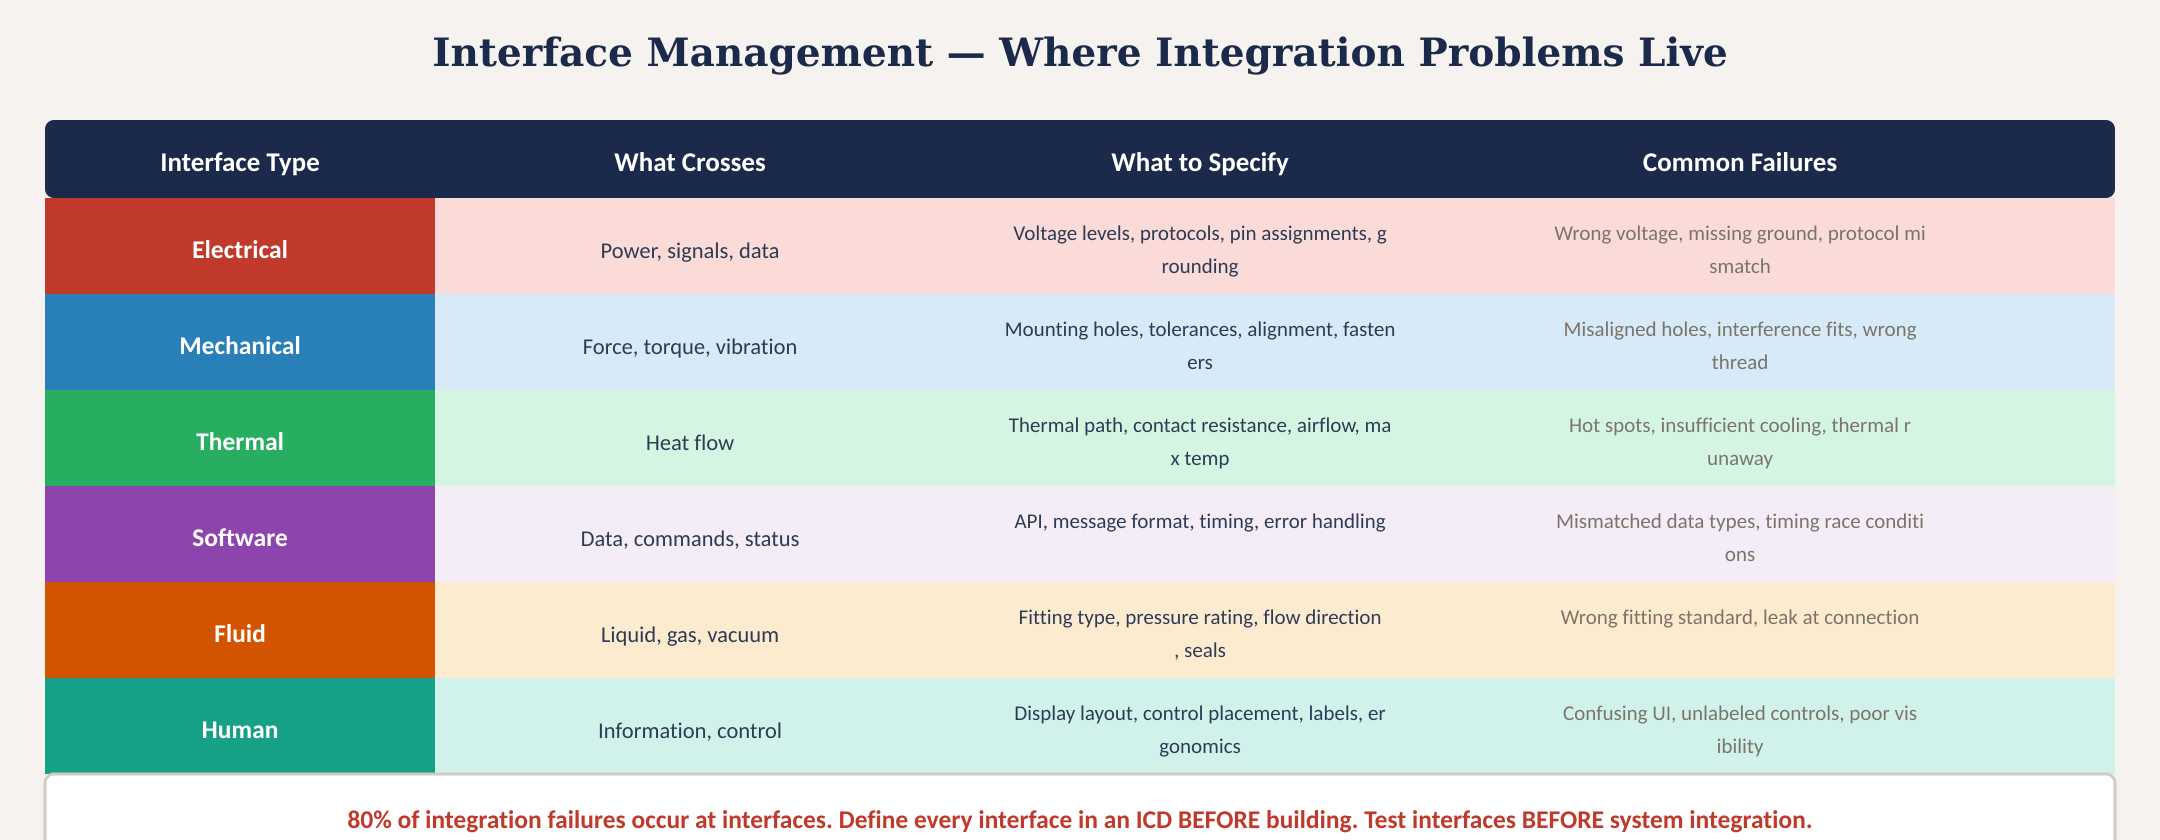
\includegraphics[width=\textwidth]{master_figs/fig_interface_management.png}
\caption{Interface types and common failure modes.}\end{figure}

\begin{figure}[htbp]\centering
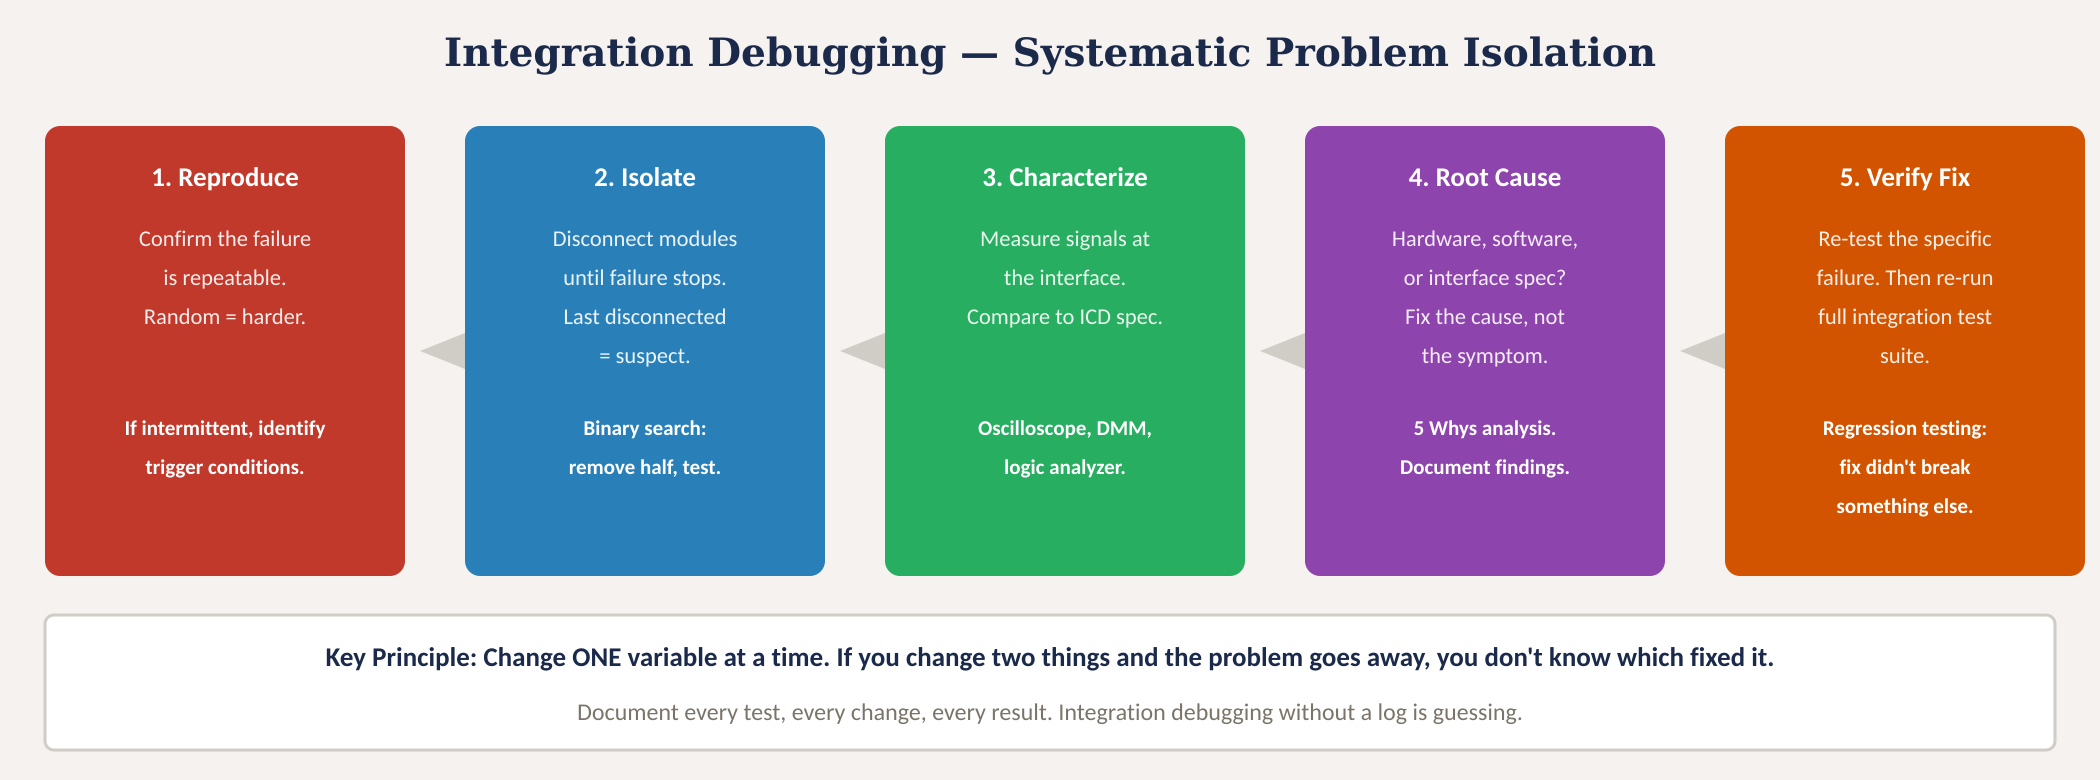
\includegraphics[width=\textwidth]{master_figs/fig_debugging_process.png}
\caption{Five-step systematic debugging process.}\end{figure}

\begin{figure}[htbp]\centering
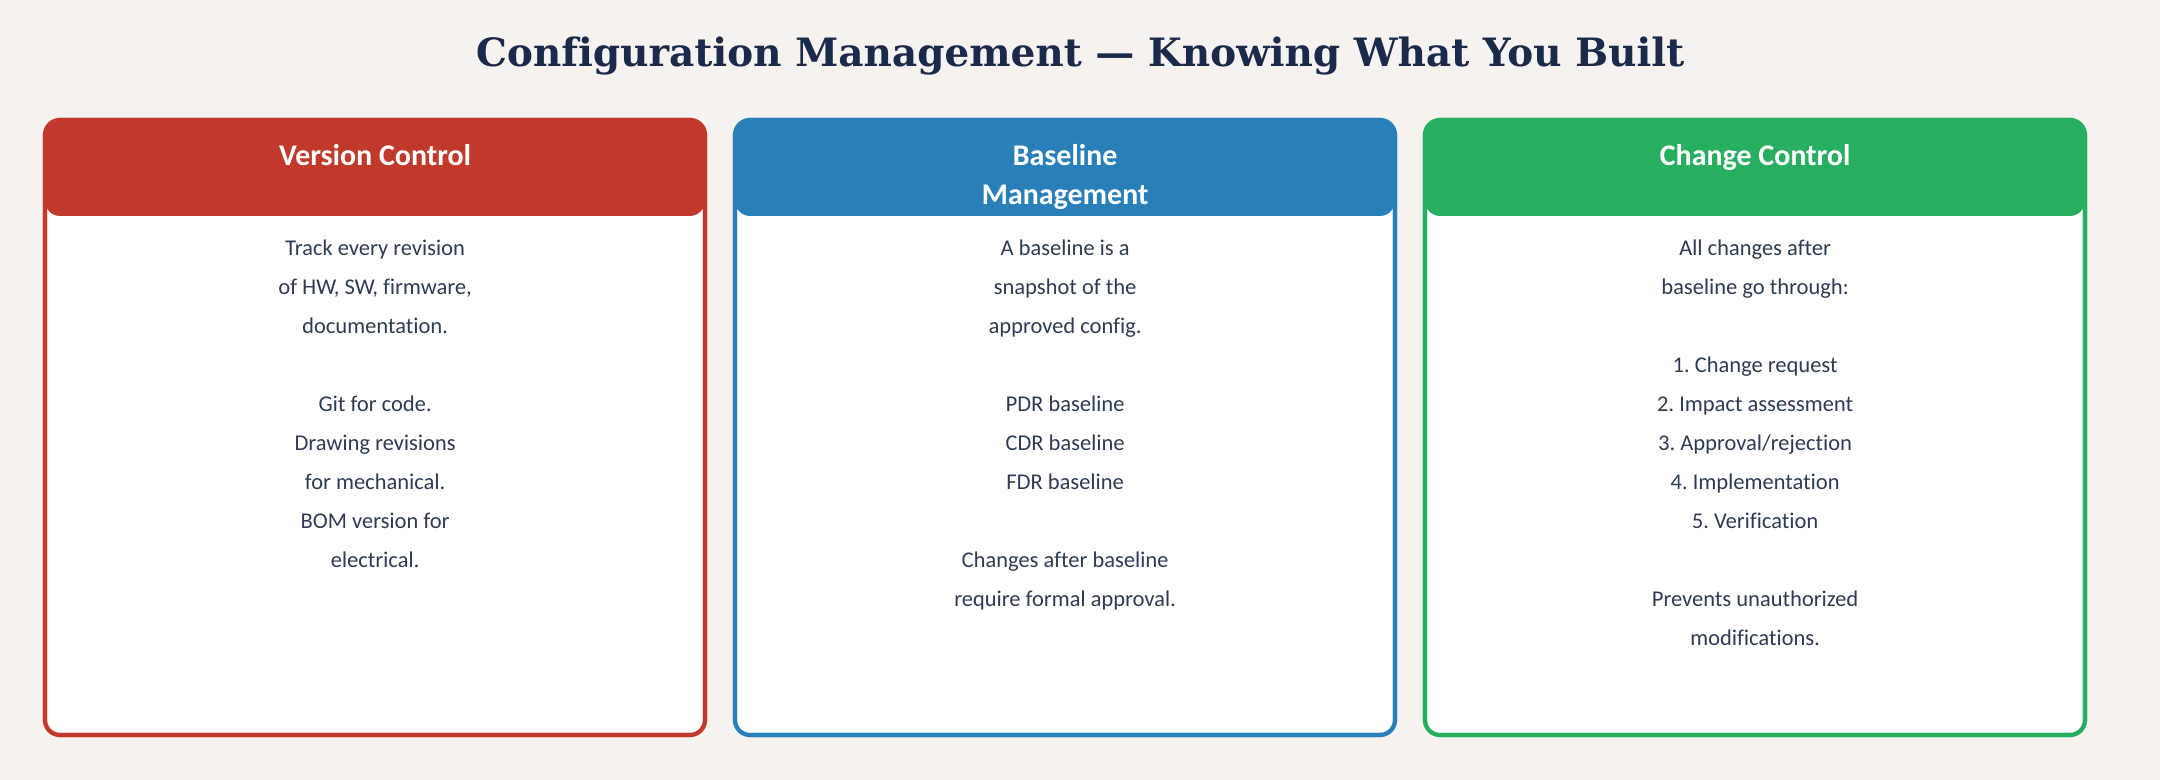
\includegraphics[width=\textwidth]{master_figs/fig_config_management.png}
\caption{Configuration management pillars.}\end{figure}

\section{Integration Strategy}
\subsection{Bottom-Up Integration}
Verify components individually $\to$ integrate into subsystems $\to$ test each subsystem $\to$ combine into system $\to$ system test. At each stage, add ONE new element and test. If something breaks, the new element or its interface is the suspect. \textbf{Never big-bang} (assemble everything at once).

\begin{figure}[htbp]\centering
\begin{tikzpicture}[
    >=Stealth,gate/.style={rectangle, draw=WarnOrange, fill=WarnOrange!15,
        text width=1.2cm, minimum height=0.6cm, align=center,
        font=\tiny\sffamily\bfseries, line width=0.6pt},
    arr/.style={->, line width=1pt, color=MinesBlue}
]
% Stages
\node[stage=MinesBlue] (c) at (0,0) {Component\\Verification};
\node[gate] (g1) at (2.4,0) {Gate 1};
\node[stage=AccentTeal] (s) at (4.8,0) {Subsystem\\Integration};
\node[gate] (g2) at (7.2,0) {Gate 2};
\node[stage=vbuild] (sys) at (9.6,0) {System\\Integration};
\node[gate] (g3) at (12.0,0) {Gate 3};
\node[stage=diagGreen] (val) at (14.4,0) {Validation};

% Flow
\draw[arr] (c) -- (g1);
\draw[arr] (g1) -- (s);
\draw[arr] (s) -- (g2);
\draw[arr] (g2) -- (sys);
\draw[arr] (sys) -- (g3);
\draw[arr] (g3) -- (val);

% Gate criteria
\node[below=0.4cm of g1,font=\tiny\sffamily,text width=2cm,align=center,MinesBlue] {Each part works alone};
\node[below=0.4cm of g2,font=\tiny\sffamily,text width=2cm,align=center,AccentTeal] {Each subsystem passes demo};
\node[below=0.4cm of g3,font=\tiny\sffamily,text width=2cm,align=center,vbuild] {VCRM all PASS};

% Never big-bang annotation
\draw[densely dashed,diagRed,line width=0.8pt] (0,-1.6) -- (14.4,-1.6);
\node[font=\tiny\sffamily\bfseries,diagRed,fill=white,inner sep=2pt] at (7.2,-1.6) {NEVER skip gates (big-bang integration)};
\end{tikzpicture}
\caption{Bottom-up integration sequence with test gates. Each gate requires all tests at the current level to pass before advancing. Skipping gates (big-bang integration) multiplies debugging time by 5--10$\times$.}\label{fig:integration_seq}
\end{figure}


\subsection{Integration Stages and the V-Model}
The V-Model maps integration from bottom-up: \textbf{Component verification} (each part works alone), \textbf{Subsystem integration} (components within a subsystem work together), \textbf{System integration} (subsystems work together), \textbf{System verification} (system meets all requirements), \textbf{Validation} (system meets stakeholder needs). Each stage has specific entry and exit criteria. Never advance with open failures.

\subsection{Integration Sequence Planning}
The order of integration matters. Rules: (1) Integrate power first; nothing works without power. (2) Add the lowest-risk subsystem next. (3) Add the highest-risk subsystem last (so problems are isolated to one new element). (4) Never add two new elements simultaneously (if something breaks, you cannot isolate the cause).

\subsection{Test Gates}
Each integration stage has entry and exit criteria. Entry: all components from the previous stage verified. Exit: all tests at the current stage PASS. Never advance with open failures.


\subsection{Critical Subsystem Demonstrations}
Before full system integration, each subsystem must pass a standalone demonstration. Three steps: (1)~\textbf{Plan}; define pass/fail criteria, (2)~\textbf{Execute}; run with data recording (video for design review), (3)~\textbf{Document}; 1-page summary with data, photos, verdict. This is a CDR deliverable.

\subsection{The N\texorpdfstring{\textsuperscript{2}}{2} (N-Squared) Diagram}
The N\textsuperscript{2} diagram maps interfaces between subsystems. Modules on the diagonal; cell $(i,j)$ = what module $i$ sends to module $j$. Dense rows/columns = high integration risk.

\begin{greenshieldbox}[GreenShield: N\textsuperscript{2} Diagram (5$\times$5)]
\small
\begin{tabularx}{\textwidth}{l|c|c|c|c|c}
 & \textbf{Sensor} & \textbf{MCU} & \textbf{Relay} & \textbf{Comms} & \textbf{PSU} \\
\hline
\textbf{Sensor} & --- & Temp (I2C) & & & \\
\hline
\textbf{MCU} & Config & --- & GPIO & UART TX & \\
\hline
\textbf{Relay} & & Status & --- & & \\
\hline
\textbf{Comms} & & UART RX & & --- & \\
\hline
\textbf{PSU} & 3.3V & 3.3V & 12V & 3.3V &; \\
\end{tabularx}

PSU interfaces with everything. MCU receives from everything. Both are high-risk integration points. The I2C bus requires defined pull-up resistor\index{pull-up resistor} ownership.
\end{greenshieldbox}

\begin{greenshieldbox}[GreenShield: I\textsuperscript{2}C Pull-Up Failure]
The sensor team assumed the MCU board had pull-ups. The MCU team assumed the sensor breakout had them. Neither did. I2C floated, communication was intermittent, 8 hours of debugging. \textbf{Fix}: every ICD must state which side provides pull-ups, termination resistors, and bias voltages.
\end{greenshieldbox}

\begin{tipbox}[Case Study: Diagnosing Brown-Out Blues]
A greenhouse controller reset randomly on relay activation. Scope showed 800\,mV dip on 3.3\,V rail (below 2.7\,V brown-out threshold). Root cause: relay coil inrush through shared power trace. Fix: 470\,$\mu$F cap on MCU rail + separate relay power trace. Regression: 100 relay cycles, zero resets.
\end{tipbox}

\begin{keyconceptbox}[Industry SE Parallels]
\begin{itemize}[nosep,leftmargin=1.5em]
\item \textbf{INCOSE SEH 4th ed.}: \S4.6 Implementation, \S4.7 Integration.
\item \textbf{NASA SP-2016-6105 Rev~2}: Ch.~5.1 Implementation, Ch.~5.2 Integration.
\end{itemize}
\end{keyconceptbox}

\section{Artifact Handoff: What Chapter 5 Produces}
\begin{table}[htbp]\centering\small
\begin{tabularx}{\textwidth}{l X l}
\toprule
\textbf{Artifact} & \textbf{Description} & \textbf{Used In} \\
\midrule
Integration Plan & Build sequence with test gates & CDR \\
N\textsuperscript{2} Diagram & Interface matrix & ICD verification \\
Integration Test Results & Subsystem and system-level data & FDR \\
\bottomrule
\end{tabularx}
\end{table}

\section{Interface Management}
80\% of integration failures occur at interfaces. Six types: electrical (voltage, protocols, grounding), mechanical (mounting, tolerances, alignment), thermal (heat flow, contact resistance), software (APIs, data formats, timing), fluid (fittings, pressure, seals), and human (displays, controls, ergonomics).

Write Interface Control Documents (ICDs) DURING architecture — not during integration. The ICD defines what crosses each boundary, in what format, with what constraints. Every interface needs a single owner.


\subsection{Interface Control Documents (ICDs)}
An ICD defines what crosses each boundary, in what format, with what constraints. Minimum ICD content for each interface:
\begin{enumerate}[nosep,leftmargin=1.5em]
\item \textbf{Interface name and number} (e.g., ICD-003: MCU $\leftrightarrow$ Relay Driver).
\item \textbf{Physical connection}: connector type, pin assignments, wire gauge/color.
\item \textbf{Electrical characteristics}: voltage levels, current draw, impedance\index{impedance}, timing.
\item \textbf{Protocol}: I2C address, baud rate, message format, error handling.
\item \textbf{Ownership}: which side provides power, pull-ups, termination.
\item \textbf{Test method}: how you verify the interface works (oscilloscope measurement, loopback test).
\end{enumerate}

Every ICD must be signed by the owners of both sides of the interface. Unsigned ICDs are the \#1 root cause of integration failures.

\section{Debugging}
Five-step process: (1) Reproduce the failure reliably. (2) Isolate by disconnecting modules until the failure stops. (3) Characterize by measuring signals at the interface against the ICD. (4) Root-cause: hardware, software, or interface spec? (5) Verify the fix, then regression-test. \textbf{Change ONE variable at a time.}

\section{Configuration Management}
Three pillars: \textbf{Version control} (Git for code, revision letters for drawings, versioned BOMs), \textbf{Baseline management} (PDR/CDR/FDR snapshots with formal change control after baseline), \textbf{Change control} (change request $\to$ impact assessment $\to$ approval $\to$ implementation $\to$ verification).


\subsection{Critical Subsystem Demonstrations}
Before full integration, each subsystem should pass a standalone demonstration. Three steps: (1) \textbf{Plan}: define what the subsystem demonstrates, test equipment needed, pass/fail criteria. (2) \textbf{Execute}: run the demonstration with data recording; video for design review. (3) \textbf{Document}: 1-page summary with data, photos, verdict; a CDR deliverable.

\section{The Integration Challenge}
Subsystem integration is where student projects most commonly fail. Each subsystem may work perfectly on the bench in isolation, but when connected together, unexpected interactions emerge: electrical noise from the motor corrupts sensor readings, the mechanical frame flexes under load and misaligns optical sensors, the firmware timing that worked with one sensor fails when three sensors share the same bus, and the power supply that was adequate for bench testing sags under full system load.

The root cause is almost always insufficient interface definition during design. If the interfaces between subsystems are not precisely specified (voltage levels, timing, mechanical tolerances, thermal limits, EMI emissions), integration becomes a process of discovering and fixing problems rather than a planned assembly.

\section{Integration Order Strategy}
\textbf{Bottom-up integration}: build and test the lowest-level components first, then assemble them into subsystems, then integrate subsystems into the full system. Advantages: problems are isolated early. Disadvantages: the full system is not tested until the end.

\textbf{Top-down integration}: start with the system-level controller and add subsystems one at a time, using stubs (simulated inputs/outputs) for subsystems not yet available. Advantages: the system architecture is validated early. Disadvantages: stubs may not represent real subsystem behavior.

\textbf{Recommended for MEGN~301}: a hybrid approach. First, integrate the ``backbone'' (power supply + MCU + communication bus). Then add subsystems one at a time, testing each integration point before adding the next. If a problem appears, it is in the most recently added subsystem or its interface.

\section{Interface Verification}
Before connecting two subsystems, verify each interface independently:

\textbf{Electrical interfaces}: measure the voltage, current, impedance, and timing at each connection point. Verify that the driving subsystem can supply what the receiving subsystem requires. Check for voltage level compatibility (3.3\,V logic vs.\ 5\,V logic), current capacity (the source can provide the load's peak current), and signal integrity (rise time, ringing, overshoot within limits).

\textbf{Mechanical interfaces}: verify that mating features align within tolerance. Check that fastener holes are concentric, that press-fit dimensions match, and that there is clearance for wire routing and assembly tools. A 0.5\,mm misalignment that is invisible on the CAD screen becomes a show-stopper during assembly.

\textbf{Software interfaces}: verify that data formats, communication protocols, timing, and error handling are consistent between subsystems. A common failure: one subsystem sends data as a 16-bit signed integer while the other expects a 32-bit float.

\section{Integration Testing Protocol}
After each subsystem is connected, execute a focused integration test:

(1) \textbf{Smoke test}: power on and verify no component overheats, no magic smoke escapes, and no fuses blow. Seriously: this catches reversed power connections, short circuits, and overcurrent conditions before they cause damage.

(2) \textbf{Communication test}: verify that the newly connected subsystem can exchange data with the controller. Send a known command; verify the expected response.

(3) \textbf{Functional test}: exercise the subsystem through its full operating range while monitoring all other subsystems for interference. Does the motor's EMI corrupt the temperature sensor? Does the pump's vibration affect the accelerometer?

(4) \textbf{Document}: record the test results, any anomalies, and the system configuration (firmware version, wiring, component values).

\section{Debugging During Integration}
When something does not work after integration, resist the urge to change multiple things simultaneously. Instead:

\textbf{Isolate}: disconnect the newly added subsystem. Does the problem persist? If yes: the problem was pre-existing (regression). If no: the problem is in the new subsystem or its interface.

\textbf{Bisect}: for the new subsystem, test each interface signal independently. Is the power supply correct? Is the communication working? Is the sensor reading plausible? Is the actuator responding?

\textbf{Instrument}: add measurement points (oscilloscope probes, serial print statements, LED indicators) to observe internal signals. The problem is almost always at an interface, and measuring the interface signals identifies which side is at fault.

\subsection{Integration Engineer's Toolkit}
Effective integration requires the right measurement tools at the bench. Know what each one does and when to reach for it:

\textbf{Multimeter}\index{multimeter}: first-reach tool. Measures DC/AC voltage, current, resistance, and continuity. Use for: verifying power rails, checking fuses, confirming wiring continuity. Limitation: cannot capture transients or timing.

\textbf{Oscilloscope}\index{oscilloscope}: essential for any time-domain problem. Use for: verifying PWM duty cycle and frequency, capturing motor inrush transients, checking I2C/SPI/UART waveforms, identifying noise and ringing on signal lines, measuring rise times. Learn to use triggering (edge, pulse width) and cursors for timing measurements.

\textbf{Logic analyzer}\index{logic analyzer}: multi-channel digital capture with protocol decode. Use for: debugging SPI/I2C/UART communication (shows exact bytes sent/received), verifying timing between multiple digital signals, capturing intermittent glitches that an oscilloscope misses. The Saleae Logic 8 (\$400) or its clones (\$15) are standard for student projects.

\textbf{Bench power supply}: not just a power source but a diagnostic tool. Use the current limit as a fault detector: set the limit to the expected current draw. If the circuit trips the limit immediately, there is a short. If it draws zero current, there is an open. The current readout tells you whether the system is behaving normally before you connect any other instruments.

\textbf{Thermal camera or IR thermometer}: identifies hot spots that indicate overcurrent, poor thermal design, or component failure. A component running 20\,\degC{} hotter than its neighbors warrants investigation. The FLIR ONE phone attachment (\$200) or a \$25 IR thermometer gun are adequate for student projects.

\begin{warningbox}[The Integration Time Estimate]
Students consistently underestimate integration time. A common estimate: ``we have 5 subsystems, each takes 1 day to build, so we need 5 days.'' Reality: building takes 5 days, but integration and debugging takes 5--15 more days. Budget at least 30\% of the total project time for integration and testing. If you have 15 weeks, reserve weeks 10--15 for integration, testing, and FDR preparation.
\end{warningbox}
\section{Interface Testing}
Before connecting two subsystems, verify each interface independently using loopback testing:

\textbf{Serial (UART) loopback}: connect TX to RX on the same device. Send a known string; verify it is received correctly. This confirms the baud rate, data format, and driver are correct before connecting to the other device.

\textbf{I2C bus scan}: use the Arduino ``I2C Scanner'' sketch to verify that each I2C device on the bus responds at the expected address. Missing devices indicate wiring errors or address conflicts.

\textbf{SPI echo}: send a known byte sequence to the SPI slave and read back the response. Verify the clock polarity, phase, and bit order match the slave's requirements.

\textbf{Power rail verification}: before connecting any subsystem to the power bus, measure the voltage and verify it is within the subsystem's input range. A 5\,V subsystem connected to a 12\,V rail is instantly destroyed.

\section{Integration Sequence for a Typical GreenShield Project}
Week 10: \textbf{Power system integration.} Connect the power supply to the distribution board. Verify all voltage rails. Connect the MCU and verify it boots. This is the ``backbone'' that everything else depends on.

Week 11: \textbf{Sensor integration.} Connect each sensor one at a time. For each: verify the raw ADC reading is plausible, apply the calibration equation, verify the engineering-unit output matches a reference measurement. If a sensor produces garbage data: check wiring, check the analog input mode (differential vs.\ RSE), check the ADC channel assignment in firmware.

Week 12: \textbf{Actuator integration.} Connect each actuator one at a time. For each: command a known output (50\% PWM\index{PWM}, fixed valve position), verify the physical response (motor spins, heater heats, valve opens). If an actuator does not respond: check the drive circuit (MOSFET gate voltage, relay coil current), check the firmware output pin assignment, verify the power supply can handle the load.

Week 13: \textbf{Control loop closure.} Connect the sensor feedback to the controller. Start with conservative gains ($K_p$ at 20\% of expected value, $K_i = 0$, $K_d = 0$). Verify the loop responds in the correct direction (negative feedback: increasing temperature reduces heater power). If the loop runs away (positive feedback): the sensor polarity or the control sign is inverted. Gradually increase gains while monitoring stability.

Week 14: \textbf{System-level testing.} Execute the formal test plan. Document results. Address non-conformances.

Week 15: \textbf{FDR preparation.} Compile test results, finalize documentation, rehearse the presentation.
\section{Practice Questions}
\begin{enumerate}[leftmargin=1.5em]
\item Your system works with subsystems A and B connected, but fails when you add subsystem C. Describe your debugging approach step by step.
\item List all interfaces for a system with a sensor module, controller board, motor driver, and power supply. Which interfaces are highest risk?
\item Your teammate changes the firmware without telling anyone and the system stops working. What configuration management\index{configuration management} failure occurred?
\item Write entry and exit criteria for the subsystem integration stage of a greenhouse monitoring system.
\item Draw an N\textsuperscript{2} diagram for a system with four modules: temperature sensor, ESP32 MCU, relay driver, and OLED display. Identify the highest-risk interface and explain why.
\item Your team skipped critical subsystem demonstrations at CDR. During integration, the motor driver outputs 5\,V logic but the MCU expects 3.3\,V. What process failure caused this, and how would a proper ICD have prevented it?
\end{enumerate}

\subsection{Answers}
\begin{enumerate}[leftmargin=1.5em]
\item Debugging approach: (1) Reproduce: confirm failure occurs with A+B+C but not A+B. (2) Isolate: is it C itself or the C-to-A/C-to-B interface? Disconnect C from B, connect only C-to-A. Does it work? Then C-to-B interface is the suspect. (3) Characterize: measure signals at the C-to-B interface against the ICD. Check voltage levels, timing, protocol. (4) Root cause: is the interface spec wrong, or is C's output wrong? (5) Fix the specific issue, re-test, then add B back.
\item Interfaces: Sensor$\leftrightarrow$Controller (I2C data + power), Controller$\leftrightarrow$Motor Driver (PWM signal + power), Motor Driver$\leftrightarrow$PSU (high-current power), Controller$\leftrightarrow$PSU (logic power), Sensor$\leftrightarrow$PSU (sensor power). Highest risk: Controller$\leftrightarrow$Motor Driver (PWM noise coupling, ground bounce from motor current spikes) and Motor Driver$\leftrightarrow$PSU (inrush current, ground loops\index{ground loop}).
\item Configuration management failure: no change control process. The teammate made an uncontrolled change. Fix: establish version control (Git for firmware), require peer review before merge, tag releases, and never deploy untested code to the integration hardware.
\item Entry criteria: all subsystem tests passed, all ICDs signed, all subsystem firmware at tagged release, test equipment available. Exit criteria: all subsystem-to-subsystem interface tests pass, system powers up and executes basic sequence, no brown-out or reset events in 30-minute soak test.
\item N$^2$ diagram: MCU column is densest (receives from all three others). MCU$\leftrightarrow$Relay Driver interface is highest risk because it crosses voltage domains (3.3\,V logic to 12\,V relay coil) and the relay switching causes noise on shared power lines.
\item The 5\,V logic on a 3.3\,V MCU input would have been caught by an ICD that specifies: ``Motor driver PWM input: 3.3\,V logic, active high, 1\,kHz.'' The ICD would have flagged the voltage incompatibility during the CDR documentation review, before any hardware was built.
\end{enumerate}


